% !TEX program = xelatex
\documentclass[]{article}
\usepackage{commons/course}

\begin{document}
\printheader

در این سوال می‌خواهیم که برنامه‌ای بنویسیم که یک
\lr{FSM}
را ورودی بگیرد و کد
\lr{control unit}
آن را به زبان
\lr{verilog}
خروجی دهد. برای این کار من از زبان
\lr{C\#} و \lr{.NET 7}
استفاده کردم.

\section*{فایل ورودی}
در ابتدا به توصیف فایل ورودی می‌پردازیم. یک نمونه از فایل ورودی در زیر و همچنین در کنار فایل اجرایی
برنامه آمده است.
\begin{latin}
\begin{lstlisting}[language=json]
{
    "inputs": ["a", "b", "c"],
    "nodes": [{
            "name": "init",
            "isAcceptState": true
        }, {
            "name": "secondry",
            "isAcceptState": false
        }, {
            "name": "blackhole",
            "isAcceptState": false
        }, {
            "name": "third",
            "isAcceptState": false
        }
    ],
    "links": [{
            "name": "a",
            "source": "init",
            "dest": "secondry"
        }, {
            "name": "c",
            "source": "secondry",
            "dest": "third"
        }, {
            "name": "c",
            "source": "third",
            "dest": "blackhole"
        }, {
            "name": "b",
            "source": "secondry",
            "dest": "blackhole"
        }
    ]
}
\end{lstlisting}
\end{latin}
این
\lr{JSON}
به کمک سایتی که آرش یادگاری زده بود بدست آمده است که صرفا کمی تفاوت کوچک با خروجی آن سایت دارد.
این سایت را می‌توانید از
\link{https://arash1381-y.github.io/fsmNinja/}{این لینک}
نگاه کنید. با این حال به بررسی هر کدام از فیلد‌های
\lr{JSON}
ورودی برنامه می‌پردازیم.
\begin{itemize}
    \item \verb|inputs|: این یک آرایه از رشته‌ است که هر کدام از فیلد‌های آن نشان دهنده‌ی ورودی مدار (\lr{control unit}) هستند. نیازی به تعریف کردن کلاک و ریست در این لیست وجود ندارد.
    \item \verb|nodes|: در این فیلد ما هر کدام از حالات \lr{FSM} را تعریف می‌کنیم. این فیلد باید یک آرایه از \lr{object} به باشد که هر کدام از آن‌ها به صورت زیر هستند:
    \begin{itemize}
        \item \verb|name|: اسم هر کدام از \lr{state}ها. دقت کنید که دو \lr{state} نباید اسم یکسانی داشته باشند.
        \item \verb|isAcceptState|: در صورتی که این مقدار برای هر یک از \lr{state}ها برابر \verb|true| باشد آنگاه آن \lr{state} حالت اولیه است. دقت کنید که فقط و تنها فقط یک حالت می‌تواند حالت اولیه باشد.
    \end{itemize}
    \item \verb|links|: در این \lr{object} باید ارتباط بین هر \lr{state} با دیگری تعریف شود. مانند \verb|nodes| این یک ارایه از \lr{object}هایی به شکل زیر است:
    \begin{itemize}
        \item \verb|name|: شرطی که باعث می‌شود که این تغییر \lr{state} رخ دهد. می‌تواند عبارت منطقی مثل \verb|a & b| نیز باشد. دقت کنید که اجزای این شرط باید در سیم‌های ورودی تعریف شده باشد.
        \item \verb|source|: تغییر \lr{state} از کدام حالت شروع می‌شود؟
        \item \verb|dest|: این تغییر \lr{state} به کدام حالت می‌رود؟
    \end{itemize}
\end{itemize}
\section*{فایل خروجی}
با دادن فایل ورودی بالا به برنامه فایل خروجی زیر درست می‌شود:
\begin{latin}
\begin{lstlisting}[language=verilog]
module GenerateModule(input wire clk, input wire reset, input wire a,input wire b,input wire c, output reg n_state, output reg p_state);
	localparam [4:0] init=4'b1000, secondry=4'b0100, blackhole=4'b0010, third=4'b0001;

	always @(*) begin
		case (p_state)
			init: begin
				if (a) begin
					n_state = secondry;
				end

			end
			secondry: begin
				if (c) begin
					n_state = third;
				end
				if (b) begin
					n_state = blackhole;
				end

			end
			blackhole: begin

			end
			third: begin
				if (c) begin
					n_state = blackhole;
				end

			end
		endcase
	end

	always @(posedge clk) begin
		if (reset)
			p_state <= init;
		else
			p_state <= n_state;
	end
endmodule
\end{lstlisting}
\end{latin}
همان طور که مشاهده می‌شود کد خروجی که تولید می‌شود علاوه بر ورودی‌های مدار که در فایل ورودی
\lr{JSON}
تعریف شده بود دو ورودی دیگر که یکی کلاک و دیگری دکمه‌ی ریست است دارد.
همچنین حالت استیت فعلی و حالت استیت بعدی نیز به عنوان خروجی در مدار قرار دارند.

در ادامه مقدار‌هایی که نشانگر حالات مختلف هستند نشان داده می‌شوند. برای نشان دادن
\lr{state}های
مختلف من از نمایش
\lr{one hot}
استفاده کردم.
سپس یک بلاک
\LRE{\verb|always @(*)|}
تعریف شده است که تعیین کردن
\lr{next state}
را بر عهده دارد. در این بلاک با توجه به حالت فعلی و سیم‌های فعال حالت بعدی مشخص می‌شود.

در نهایت نیز یک بلاک
\LRE{\verb|always @(posedge clk)|}
وجود دارد که وظیفه‌ی مقداردهی
\lr{next state} و ریست
را در هر کلاک بر عهده دارد.

\section*{اجرای برنامه}
برای اجرای برنامه کافی است که فایل
\verb|FSM-To-Verilog.exe|
را همراه با اسم فایل ورودی
\lr{json}
که تعریف
\lr{FSM}
است را اجرا کنیم. فایل خروجی
\verb|output.v|
در کنار برنامه ساخته می‌شود که خروجی ما است.
در شکل زیر یک نمونه اجرای برنامه را مشاهده می‌کنید.
\begin{figure}[ht]
    \centering
    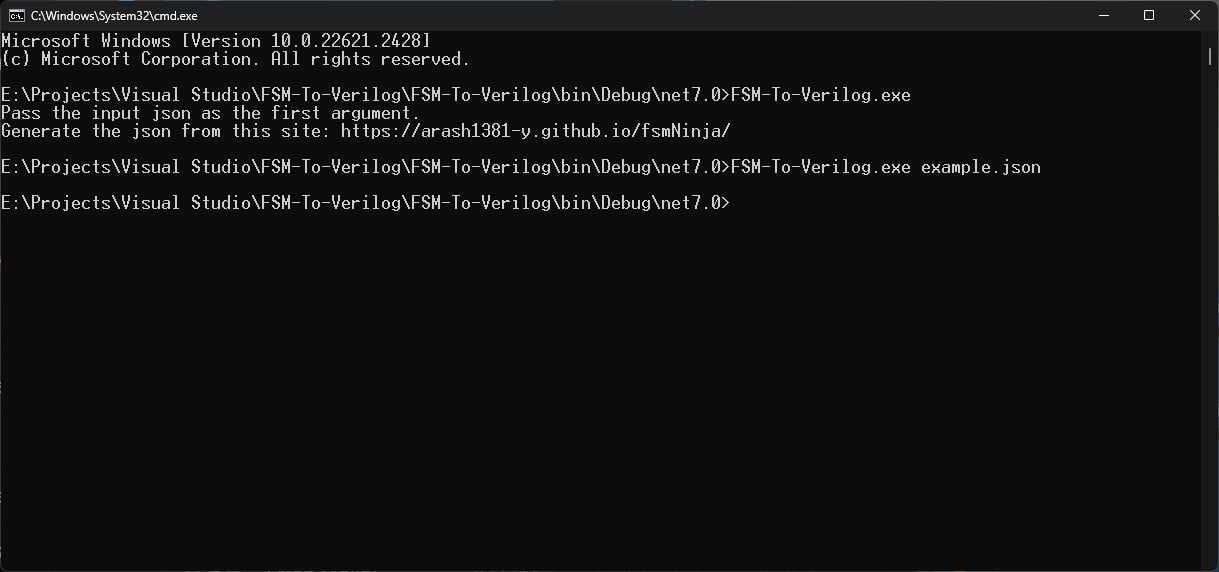
\includegraphics[scale=0.4]{pics/run.jpg}
\end{figure}
در فایل آپلودی فایل برنامه‌ی کامپایل شده در فولدر
\lr{bin}
قرار دارد.

\section*{کامپایل برنامه}
برای کامپایل برنامه شما نیاز به
\lr{.NET 7}
خواهید داشت. بعد از نصب آن کافی است که خط زیر را در دایرکتوری پروژه اجرا کنید:
\begin{latin}
\begin{lstlisting}[language=verilog]
dotnet build
\end{lstlisting}
\end{latin}
\end{document}
